
% vim: set nospell nowrap textwidth=0 wrapmargin=0 formatoptions-=t:
\RequirePackage[l2tabu,orthodox]{nag}
\documentclass{standalone}
\usepackage{lmodern}
% \usepackage[paperwidth=182mm,paperheight=220mm,margin=0.02in,heightrounded,landscape]{geometry}
\usepackage{tikz}
\usetikzlibrary{positioning, fit, calc, arrows.meta, intersections, backgrounds, shapes, decorations.pathreplacing, decorations.markings}
\usepackage{mathtools}
\usepackage{circuitikz}
% \usepackage[center,pdflatex,frame]{crop}

\definecolor{lightgrey}{rgb}{0.918,0.929,0.929}
\definecolor{stilllightergrey}{rgb}{0.959,0.9645,0.9645}
\definecolor{coolgrey}{rgb}{0.6156,0.6156,0.6156}
\definecolor{darkergrey}{rgb}{0.3078,0.3078,0.3078}
\definecolor{intermediategrey}{rgb}{0.7668,0.7723,0.7723}
\definecolor{lightblue}{rgb}{0.831,0.937,0.988}
\definecolor{lightgreen}{rgb}{0.6,0.847,0.7882}
\definecolor{imperialblue}{rgb}{0,0.243,0.455}
\definecolor{lime}{rgb}{0.7686,0.8392,0}
\definecolor{darkteal}{rgb}{0.05882,0.5098,0.5686}
\definecolor{darkgreen}{rgb}{0.00784,0.53725,0.23137}
\definecolor{orange}{rgb}{0.8235,0.25098,0}
\definecolor{lemonyellow}{rgb}{1,0.847058,0.003921}
\definecolor{poolblue}{rgb}{0.047,0.631,0.803}
\definecolor{processblue}{rgb}{0,0.52156,0.79215}
\definecolor{seaglass}{rgb}{0.215,0.623,0.623}
\definecolor{teal}{rgb}{0,0.556786,0.666}
\definecolor{imperialmoddedblue}{rgb}{0,0.43137,0.68627}
\definecolor{brick}{rgb}{0.64705,0.098039,0}
\definecolor{imperialmoddedred}{rgb}{0.8667,0.14509,0.00392}
\definecolor{imperialmoddedviolet}{rgb}{0.588235,0,0.470588}
\definecolor{iris}{rgb}{0.466667,0.145098,0.513725}
\definecolor{magentapink}{rgb}{0.784314,0.117647,0.470588}
\definecolor{raspberry}{rgb}{0.568627,0,0.282353}
\definecolor{cherry}{rgb}{0.835294,0,0.196078}
\definecolor{tangerine}{rgb}{0.92549,0.45098,0}
\definecolor{darkgreen}{rgb}{0.007843,0.537255,0.231373}
\definecolor{kermitgreen}{rgb}{0.4,0.643137,0.039216}

\begin{document}
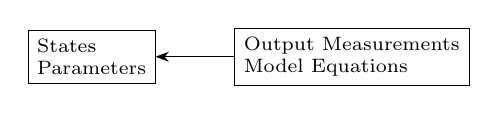
\begin{tikzpicture}[every node/.style={draw,very thin, align=left,{font=\scriptsize}},>=Stealth]
    % \node (leastsquares){Least\\Squares};
    % \node [right = of leastsquares] (probabilitytheory){Probability\\Theory};
    % \node [right = of probabilitytheory] (dynamicsystems) {Dynamic\\Systems};
    % \node [fit=(leastsquares.north)(probabilitytheory.north),above=of leastsquares,anchor=south west,inner sep=0pt] (lms) {Least Mean\\Squares};
    % \node [fit=(dynamicsystems.north)(probabilitytheory.north),above=of dynamicsystems,anchor=south east,inner sep=0pt] (stochastic) {Stochastic\\Systems};
    % \node [fit=(lms.north)(stochastic.north),above=of stochastic,anchor=south east,inner sep=0pt] (kf) {Kalman\\Filtering};

    \node (inverseproblem) {States\\Parameters};
    \node [ right = 10mm of inverseproblem] (inverseprobleminput) {Output Measurements\\Model Equations};
    \draw [<-] (inverseproblem) -- (inverseprobleminput);
\end{tikzpicture}
\end{document}